\renewcommand{\thechapter}{2}

\chapter{Laser cooling and trapping of neutral atoms}

The Nobel Lecture of W.D.Phillips, {\it Laser cooling and trapping of neutral atoms} \cite{phillips1998nobel} tells a great story of the development of laser cooling techniques since the late 1970s. It is recommended for readers who want to learn not only the development of the laser cooling research field but also how researchers approach new physics and technology in a close view. It is aspiring to learn the mature technology that cold atom researcher uses on a daily basis to expand the boundary of physics results from the intelligence, efforts, and persistent pursuit of the early generation of physicists.    

Laser cooling techniques eventually lead to the observation of BEC in 1995, the first Bose-Einstein condensate was created by Eric Cornell, Carl Wieman, and co-workers at JILA on 5 June 1995 \cite{anderson1995observation}. They cooled a dilute vapor of approximately two thousand $^{87} {\rm Rb}$ atoms to below 170~ ${\rm nK}$ using a laser cooling and magnetic evaporative cooling. About four months later, an independent effort led by Wolfgang Ketterle at MIT condensed $^{23} {\rm Na}$ \cite{davis1995bose}. The observation of BEC won laser cooling pioneers Steven Chu, Claude Cohen-Tannoudji, and William D. Phillips the 1997 Nobel Prize in Physics. And Cornell, Wieman, and Ketterle won the 2001 Nobel Prize in Physics for their achievements.

After more than twenty years, the research field of cold atoms is prosperous. The development of laser cooling techniques and the methods to make stable BEC have not only achieved a new state of matter predicted only by Quantum physics, the highly controllable optical and magnetic potential, tunable interaction between particles, and precision measurement techniques have made the BEC system a great platform for Quantum simulation and Quantum computation. 

In this chapter, we use $^{87} {\rm Rb}$ as an example. Start from its energy level, its interaction with light and magnetic field, and then discuss the laser cooling techniques that are essential to make BEC.  

\section{Hyperfine Structures}

\subsection{Energy Level Splitting}
The energy splitting of $^{87} {\rm Rb}$ ground state and the first excited state can be found in Fig.~(\ref{fig:D1andD2}) from \cite{steck2001rubidium}, it is a great source of $^{87} {\rm Rb}$ D lines data.

For the ground state of $^{87} {\rm Rb}$, the quantum number of orbital angular momentum ${\bf L}$ is 0 and the first excited state $L = 1$. When we consider the spin of the single electron in the outer shell of the atom, $S = 1/2$, and the interaction between spin and orbital angular momentum ${\bf L} \cdot {\bf S}$, the excited state splits into a fine-structure doublet. The eigenvalue of total electron angular momentum 
\begin{equation}
    {\bf J} = {\bf L} + {\bf S}    
\end{equation}
becomes a good quantum number. For the ground state,  $L = 0$, $S = 1/2$, and $J = 1/2$. The ground state is labeled as $5^2S_{1/2}$ where the atomic states are described by term symbols of the form
\begin{equation}
    ^{2S+1}L_J.
\end{equation}
The interaction between the spin and the orbital angular momentum splits the excited state into doublet $5^2P_{1/2}$ and $5^2P_{3/2}$. The transition between the ground state and the excited state is split into two lines, D1 line($5^2S_{1/2} \rightarrow 5^2P_{1/2}$) and D2 line ($5^2S_{1/2} \rightarrow 5^2P_{3/2}$).

Accounting for nuclear angular momentum ${\bf I}$, the states further split into hyperfine states and are represented in the basis of the total angular momentum
\begin{equation}
    {\bf F} = {\bf J} + {\bf I}.    
\end{equation}
The quantum number of the nuclear spin of $^{87} {\rm Rb}$ is 3/2, as shown in Fig.~(\ref{fig:D1andD2}), the $^{87} {\rm Rb}$ ground state $5^2S_{1/2}$ splits into hyperfine states $\ket{F=1}$ and $\ket{F=2}$. The excited state $5^2P_{1/2}$ splits into hyperfine states $\ket{F=1}$ and $\ket{F=2}$. And the excited state $5^2P_{3/2}$ splits into hyperfine states $\ket{F=1}, \ket{F=2},\ket{F=3}$ and $\ket{F=4}$. The Hamiltonian that leads to the hyperfine split consists of magnetic dipole interaction and electric quadrupole interaction,
\begin{equation}
    \hat{H}_{hfs} = A_{hfs}{\bf I}\cdot{\bf J} + B_{hfs}\frac{3({\bf I}\cdot{\bf J})^2 + 3/2{\bf I}\cdot{\bf J} - I(I+1)J(J+1)}{2I(2I-1)2J(2J-1)}.
\end{equation}
Here $A_{hfs}$ is the magnetic dipole constant and $B_{hfs}$ is the electric quadrupole constant. The hyperfine energy splits for the states are
\begin{equation}
    \Delta E_{hfs} = \frac{1}{2}A_{hfs}K + B_{hfs}\frac{3/2K(K+1) - 2I(I+1)J(J+1)}{2I(2I-1)2J(2J-1)}
\end{equation}
where 
\begin{equation}
    K = F(F+1) - I(I+1) - J(J+1).
\end{equation}
The numerical results of hyperfine states energy can be found in Fig.~(\ref{fig:D1andD2}), they are calculated given the experimental measurement of $A_{hfs}$ and $B_{hfs}$ \cite{bize1999high,ye1996hyperfine,barwood1991frequency}.
\begin{figure}[htbp]
    \centering
    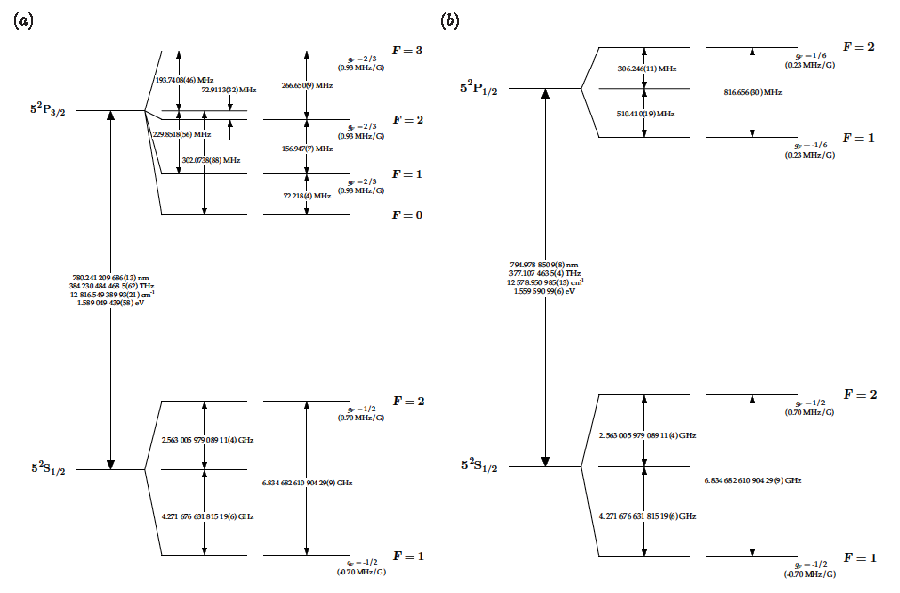
\includegraphics[width=\textwidth]{Chapter2_secs/D1andD2.pdf}
    \caption{Energy splitting of the $^{87} {\rm Rb}$ ground state and the first excited state. }
    \label{fig:D1andD2}
\end{figure}
\subsection{Zeeman splitting of $^{87} {\rm Rb}$ hyperfine ground states}\label{zeeman chpt}
The angular momentum of $^{87} {\rm Rb}$ interacts with the external magnetic field and the hyperfine states split into sub-states. Here we use perturbation theory to calculate the energy of each sub-states of $^{87} {\rm Rb}$ ground state.

For the $^{87} {\rm Rb}$ ground state, $J=1/2$ and $I=3/2$. It has hyperfine states $\ket{F=1}$ and $\ket{F=2}$. The Hamiltonian with external magnetic field is 
\begin{equation}
    \hat{H} = \hat{H}_{hfs} + (\mu_B g_J\Vec{J} + \mu_N g_I\Vec{I})\Vec{B}.
\end{equation}
Here $\mu_B = 9.27\times 10^{-24} {\rm J}\cdot {\rm T}^{-1}$ is Bohr magneton, the natural unit for expressing the magnetic moment of an electron caused by either its orbital or spin angular momentum. $\mu_N = 5.05\times 10^{-27} {\rm J}\cdot {\rm T}^{-1}$ is the nuclear magneton. $g_J$ and $g_I$ are land\'e g-factors. For $^{87} {\rm Rb}$ ground state, $g_J \approx 2.00233$ and $g_I \approx -0.00099$. 

Define the direction of magnetic field z, the Hamiltonian can be represented by the z-component of angular momentum
\begin{equation}
    \hat{H} = \hat{H}_{hfs} + \mu_B(g_J m_J + g_Im_I)B,
\end{equation}
where $m_J$ and $m_I$ are magnetic quantum numbers. $\hat{H}_{hfs}$ is diagonal in the basis of $\{\ket{F,m_F}\}$, and we can proceed by representing states $\ket{J=1/2,m_J,I=3/2,m_I}$ with $\{\ket{F,m_F}\}$ and calculate the energy of states $\ket{F,m_F}$ to second order.

\begin{align}
    &\ket{\frac{1}{2},\frac{3}{2}} = \ket{2,2}, &&\ket{\frac{1}{2},\frac{1}{2}} = \frac{\sqrt{3}}{2}\ket{2,1} - \frac{1}{2}\ket{1,1}\\\nonumber
    &\ket{\frac{-1}{2},\frac{3}{2}} = \frac{1}{2}\ket{2,1} + \frac{\sqrt{3}}{2}\ket{1,1}, &&\ket{\frac{-1}{2},\frac{1}{2}} = \frac{1}{\sqrt{2}}\ket{2,0} + \frac{1}{\sqrt{2}}\ket{1,0}\\ \nonumber
    &\ket{\frac{1}{2},\frac{-1}{2}} = \frac{1}{\sqrt{2}}\ket{2,0} - \frac{1}{\sqrt{2}}\ket{1,0}, &&\ket{\frac{1}{2},\frac{-3}{2}} = \frac{1}{2}\ket{2,-1} - \frac{\sqrt{3}}{2}\ket{1,-1}\\ \nonumber
    &\ket{\frac{-1}{2},\frac{-1}{2}} = \frac{\sqrt{3}}{2}\ket{2,-1} - \frac{1}{2}\ket{1,-1}, &&\ket{\frac{-1}{2},\frac{-3}{2}} = \ket{2,-2}\\ \nonumber
\end{align}

In the $\{\ket{F,m_F}\}$ basis,
\begin{equation}
    \hat{H}_{hfs}\ket{F,m_F} = E_{F}\ket{F,m_F}.
\end{equation}
Treat the interaction with the external magnetic field as a perturbation, the first-order perturbed energy for state $\ket{F,m_F}$ is
\begin{equation}
    \Delta E_1 = \matrixel{F,m_F}{(g_J\Vec{J}_z + g_I\Vec{I}_z)}{F,m_F}\mu_B B,
\end{equation}
and the second order perturbed energy is
\begin{equation}
    \Delta E_2 = \sum_{F',m_F'} \frac{|\matrixel{F,m_F}{(g_J\Vec{J}_z + g_I\Vec{I}_z)}{F',m_F'}|^2}{E_F-E_{F'}}(\mu_B B)^2.
\end{equation}

The energy of $\ket{F,m_F}$ states are listed here, in the units of ${\rm MHz}$, ${\rm MHz/G}$ and ${\rm MHz/G^2}$. The numbers are useful for quick estimation of the magnetic field in the lab.
\begin{align}
    \ket{2,2} &= 2.75\times 10^3h ~{\rm MHz} + 1.405h~{\rm MHz/G}\times B + 0h ~{\rm MHz/G^2}\times B^2\\\nonumber
    \ket{2,1} &= 2.75\times 10^3h ~{\rm MHz} + 0.7026h~{\rm MHz/G}\times B + 2.879\times 10^{-4}h ~{\rm MHz/G^2}\times B^2\\\nonumber
    \ket{2,0} &= 2.75\times 10^3h ~{\rm MHz} + 0h~{\rm MHz/G}\times B + 3.839\times 10^{-4}h ~{\rm MHz/G^2}\times B^2\\\nonumber
    \ket{2,-1} &= 2.75\times 10^3h ~{\rm MHz} - 0.7026h~{\rm MHz/G}\times B + 2.879\times 10^{-4}h ~{\rm MHz/G^2}\times B^2\\\nonumber
    \ket{2,-2} &= 2.75\times 10^3h ~{\rm MHz} - 1.405h~{\rm MHz/G}\times B + 0h ~{\rm MHz/G^2}\times B^2\\\nonumber
    \ket{1,1} &= -4.2896\times 10^3h ~{\rm MHz} - 0.7052h~{\rm MHz/G}\times B - 2.879\times 10^{-4}h ~{\rm MHz/G^2}\times B^2\\\nonumber
    \ket{1,0} &= -4.2896\times 10^3h ~{\rm MHz} + 0h~{\rm MHz/G}\times B - 2.879\times 10^{-4}h ~{\rm MHz/G^2}\times B^2\\\nonumber
    \ket{1,-1} &= -4.2896\times 10^3h ~{\rm MHz} + 0.7052h~{\rm MHz/G}\times B - 2.879\times 10^{-4}h ~{\rm MHz/G^2}\times B^2\\\nonumber
\end{align}

The second-order perturbation leads to the quadratic Zeeman shift which has a sizable effect when the magnetic field on the order of $ 10{\rm G}$. In some our experiments, the quadratic Zeeman shift makes the energy difference between $\ket{1,0}$ and $\ket{1,-1}$ large enough than the difference between $\ket{1,0}$ and $\ket{1,1}$. So we can effectively treat the $F=1$ manifold as a two-level system by decoupling $\ket{1,-1}$. 

For larger magnetic field, larger than $10^3{\rm G}$, the perturbation theory breaks down and {\bf Breit-Rabi formula} \cite{breit1931measurement} is useful in the case $J=1/2$. 
\begin{align}
     &E_{F=I\pm1/2} = -\frac{A_{hfs}}{4} + m_Fg_I\mu_NB \pm A_{hfs}\sqrt{1 + m_Fx x^2}, m_F \neq 2, -2\\ \nonumber
     &E_{F=2,m_F=\pm2} = -\frac{A_{hfs}}{4} + m_Fg_I\mu_NB + A_{hfs}(1 \pm x) \\\nonumber
     &x = \frac{(g_J\mu_B - g_I\mu_N)B}{2A_{hfs}}\\\nonumber
\end{align}
The energy of states $\ket{F,m_F}$ is shown in Fig.~(\ref{fig:BField}) for the magnetic field up to 15000 {\rm G}.

\begin{figure}[htbp]
    \centering
    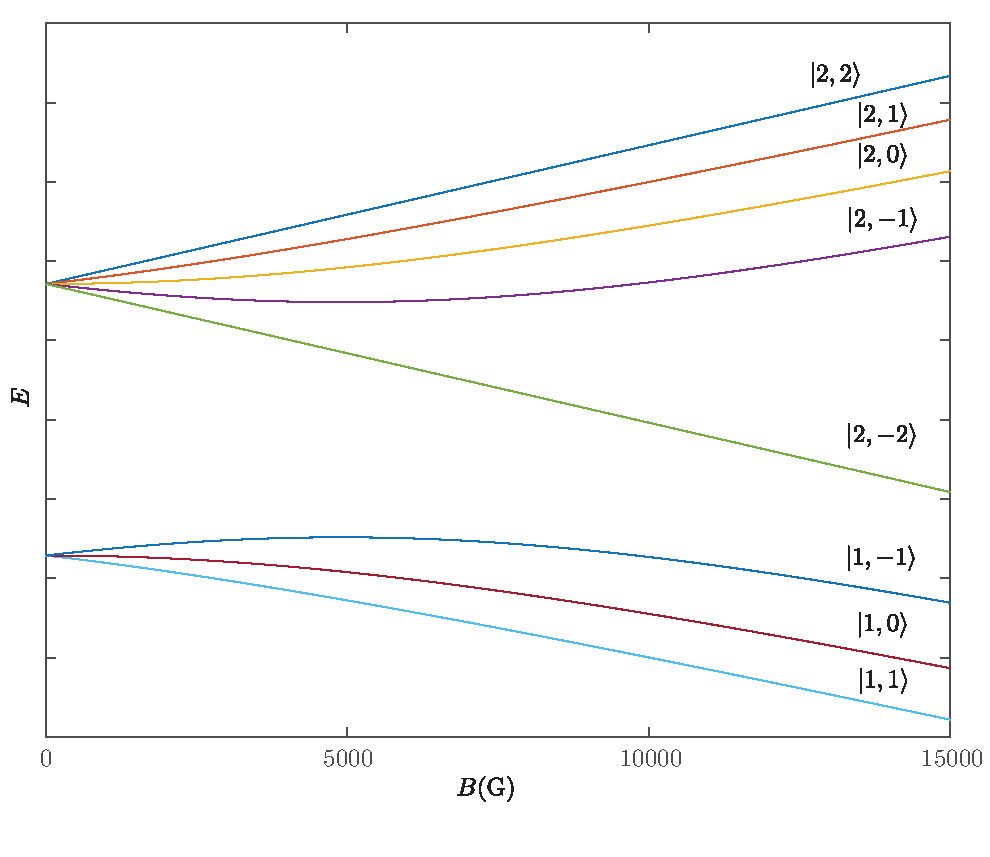
\includegraphics[width=\textwidth]{Chapter2_secs/B_field.pdf}
    \caption{Zeeman splitting of $^{87} {\rm Rb}$ ground states $\ket{F,m_F}$. }
    \label{fig:BField}
\end{figure}

\section{Laser cooling techniques}

\subsection{Two level system interacting with reservoir}

\begin{figure}[htbp]
    \centering
    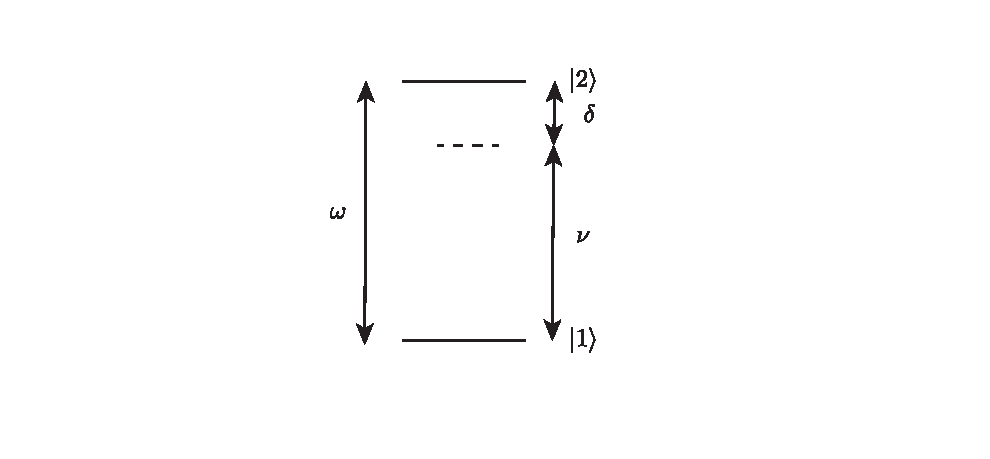
\includegraphics[width=\textwidth]{Chapter2_secs/twolevel.pdf}
    \caption{A two level system with energy difference $\omega$ in a light field with frequency $\nu$. $\delta = \nu - \omega$ is the detuning. }
    \label{fig:twolevel}
\end{figure}
A two level system shown in Fig.~(\ref{fig:twolevel}) interacts with light field via electric dipole interaction. 
\begin{equation}
    \hat{H} = -\Vec{d}\cdot \Vec{E}
\end{equation}
is the electric dipole interaction Hamiltonian where $\Vec{d} = e\Vec{r}$ is the dipole operator. The matrix element of dipole operator $\matrixel{L',m_L'}{\Vec{d}}{L,m_L}$ is nonzero only when $\Delta L = \pm 1$ and $\Delta m_L = 0$. The dipole operator doesn't interact with spin and nuclear angular momentum, so in the total angular momentum basis, the selection rule is 
\begin{equation}
    \Delta F = \pm 1.
\end{equation}
The Electric field
\begin{equation}
    \Vec{E} = E_x {\bf e_x} + E_y {\bf e_y} + E_z {\bf e_z}
\end{equation}
can be expressed in the basis of $\{ {\bf e_{\pm}},{\bf e_z}\}$,
\begin{equation}
    \Vec{E} = E_+ {\bf e_+} + E_- {\bf e_-} + E_z {\bf e_z}.
\end{equation}
Here,
\begin{equation}
    {\bf e_{\pm}} = \frac{{\bf e_x} \pm i{\bf e_y}}{\sqrt{2}}.
\end{equation}
The dipole interaction Hamiltonian is separated into the radial part and the angular part in the new basis,
\begin{equation}
    {\bf e_q}\cdot \Vec{r} = \sqrt{\frac{4\pi}{3}}\rho Y_{1,q}(\theta,\phi),
\end{equation}
here q = 1 for ${\bf e_+}$, q = -1 for ${\bf e_-}$ and q = 0 for ${\bf e_z}$, $Y_{1,q}(\theta,\phi)$ is the spherical harmonic function.

A two level system with energy difference $\omega$ interacts with electromagnetic field
\begin{equation}
    \Vec{E}(\Vec{r},t) = \Vec{E}_0 e^{-i(\nu t-\Vec{k}\cdot\Vec{r})} + \Vec{E}_0^*e^{i(\nu t-\Vec{k}\cdot\Vec{r})},
\end{equation}
the Hamiltonian is
\begin{equation}
    \hat{H} = \hbar \omega \dyad{2}{2} - (\Vec{\mu} \dyad{1}{2} + \Vec{\mu}^*\dyad{2}{1})\cdot\Vec{E}(\Vec{r},t).
\end{equation}
By transforming into a rotating frame, 
\begin{equation}
    \ket{\Tilde{2}} = e^{i\nu t}\ket{2},
\end{equation}
and neglecting the fast oscillating term $e^{\pm i\nu t}$, the Hamiltonian is transformed to
\begin{equation}
    \hat{H} = \hbar\delta \dyad{\Tilde{2}}{\Tilde{2}} + \hbar(\Omega \dyad{1}{\Tilde{2}} + \Omega^* \dyad{\Tilde{2}}{1}),
\end{equation}
Here,
\begin{equation}
    \Omega = \frac{\Vec{E}_0 \cdot \Vec{\mu}}{\hbar}.
\end{equation}
The frame transformation and the removal of the oscillating term is named after rotating wave approximation (RWA), it is widely used in atomic physics when atoms interact with near resonance high frequency optical field, and satisfying the condition $\delta \ll \nu, \omega$.

The Hamiltonian above describes a closed system, where the two level atom only interacts with the one single optical mode and the evolution of atomic states and photon states is coherent. In reality, the atom interacts not only with the optical field but also the vacuum modes in the environment. The vacuum modes are contiguous in free space and discrete in a cavity, the coupling between the atomic states to the vacuum modes leads to spontaneous emission of the excited state and causes incoherence. Wigner-Weisskopf theory \cite{scully1999quantum} represents the vacuum modes with quantized field operators and calculates spontaneous emission with Fermi's golden rule. The Hamiltonian of atomic system and vacuum modes is
\begin{equation}
    \hat{H} = \hbar \omega \dyad{2}{2} + \sum_j\hbar \nu (\hat{a}^\dag_j\hat{a}_j + \frac{1}{2}) - \sum_j(\hbar g_j \dyad{2}{1}\hat{a}_j + \hbar g_j^* \dyad{1}{2}\hat{a}^\dag_j),
\end{equation}
and $g_j$ is the coupling strength between the states $\ket{2,0}$ and $\ket{1,1_k}$. $\ket{1,1_k}$ is the state with one photon occupying mode $k$.
\begin{equation}
    \gamma = 2\pi \sum_j |g_j|^2\delta(\nu_j - \omega)
\end{equation}
is the result of spontaneous emission rate $\gamma$ and in free space
\begin{equation}
    \gamma = \frac{\omega^3|\mu|^2}{3\pi\epsilon_0\hbar c^3},
\end{equation}
which is also known as the Einstein A coefficient.

One way to describe both coherent and incoherent evolution is using density operator. The density operator is defined as
\begin{equation}
    \hat{\rho} = \sum_\alpha p_\alpha \dyad{\phi_\alpha}{\phi_\alpha}.
\end{equation}
Here, $\ket{\phi_\alpha}$ a quantum state and $p_\alpha$ is the probability that the state is in $\ket{\phi_\alpha}$. The states $\ket{\phi_\alpha}$ are not necessarily orthogonal to each other, but for the density operator representation to be valid, it has to satisfy the following condition,
\begin{equation}
    {\rm Tr}[\hat{\rho}] = 1.
\end{equation}
For any orthonormal basis $\{ \ket{n}\}$, 
\begin{equation}
    \sum_n \matrixel{n}{\hat{\rho}}{n} = 1,  and ~ {\rm Tr}[\hat{\rho}] = \sum_n \matrixel{n}{\hat{\rho}}{n},
\end{equation}
for the conservation of probability.

In the density operator representation, the expectation value of a dynamic variable $\hat{A}$ can be calculated using
\begin{equation}
    \expval{\hat{A}} = {\rm \hat{\rho}\hat{A}}.
\end{equation}

In the orthonormal basis $\{ \ket{n}\}$, the matrix element of the density operator is
\begin{equation}
    \rho_{n,n'} = \matrixel{n}{\hat{\rho}}{n'}.
\end{equation}
The diagonal elements $\rho_{n,n}$ represents the the probability that the state is in $\ket{n}$ and the off-diagonal elements $\rho_{n,n'}$ represents the expectation value of coherence between states $\ket{n}$ and $\ket{n'}$. If there exists a state $\ket{\phi}$ such that
\begin{equation}
    \hat{\rho} = \dyad{\phi}{\phi},
\end{equation}
the state represented by $\hat{\rho}$ is a pure state, otherwise, it is a mixed state. In quantum mechanics, the probability amplitude of states bear the full information, probability and coherence. The density operation representation loses the information of coherence of some states but the expectation value of coherence is preserved. 

For an open system, the physical system we are interested in interacts with the environment, or sometimes called reservoir. The reservoir can contain a large number of degrees of freedom, for example, vacuum modes and other electromagnetic fields modes. The large number of degrees of freedom of the reservoir makes it hard to study its dynamics, however, in many cases, we are not actually interested in learning about the evolution of the reservoir. In these cases, it is useful to ignore the dynamics of the reservoir and only keep the effect the reservoir has on the system. By making this assumption, the coherent evolution of the system and the reservoir is lost and there exists decoherence in the dynamic of the system, so density operator is widely used to describe the open system.

The full Hamiltonian is
\begin{equation}
    \hat{H} = \hat{H}_S +\hat{H}_R + \hat{H}_{SR} 
\end{equation}
and under Heisenberg's equation, the evolution of the density operator is
\begin{equation}
    \frac{d}{dt}\hat{\rho} = \frac{1}{i\hbar}\left[ \hat{H},\hat{\rho} \right]
\end{equation}
Assume the interaction operator takes the form
\begin{equation}
    \hat{H}_{SR}  = \hat{S}\hat{R}^\dag + \hat{S}^\dag\hat{R}.
\end{equation}
To ignore the dynamics of the reservoir and only keep the effects it has on the system, we need to make two assumptions. First, factorize the reservoir operator
\begin{equation}
    \hat{R} \approx f(t)\hat{\Tilde{R}}.
\end{equation}
The function $f(t)$ characterizes the time evolution of the reservoir, and it is often assumed that the reservoir is stationary in the stochastic process language. The auto-correlation function of $f(t)$ is defined as
\begin{equation}
    ACF_f(t-t') = \expval{(f(t)-\expval{f(t)})(f(t')-\expval{f(t')})}.
\end{equation}
The correlation time $t_c$ of the function $f(t)$ is defined as the width of the peak of $ACF_f(t-t')$. 
The first assumption of reservoir is that $t_c \ll 1$, which means the reservoir has Markovian property, it quickly forgets about its previous state does not keep the memory of interacting with the system.

The second assumption is the reservoir is large enough that the system can hardly affect its state. Again, this means that the reservoir is stationary. Under these assumptions, the dynamics of the system is derived and expressed in terms of the reduced density operator
\begin{equation}
    \hat{\rho}_S = {\rm Tr}_{\rm R} [\hat{\rho}],
\end{equation}
which takes the average of the reservoir state by tracing out the reservoir degrees of freedom.

For a two level system
\begin{equation}
    \hat{H}_S = \hbar\delta \dyad{2}{2} + \hbar(\Omega \dyad{1}{2} + \Omega^* \dyad{2}{1}),
\end{equation}
the density operator evolves under eqaution
\begin{align}\label{OBE}
    &\dot{\rho}_{22} = -\gamma(\overline{n} + 1)\rho_{22} + \gamma\overline{n}\rho_{11} + i\Omega^*\rho_{21} - i\Omega\rho_{12}\\\nonumber
    &\dot{\rho}_{11} = \gamma(\overline{n} + 1)\rho_{22} - \gamma\overline{n}\rho_{11} - i\Omega^*\rho_{21} + i\Omega\rho_{12}\\\nonumber
    &\dot{\rho}_{12} = -\frac{\gamma}{2}(2\overline{n} + 1)\rho_{12} - i\delta\rho_{12} - i\Omega^*(\rho_{22}-\rho_{11})\\\nonumber
    &\dot{\rho}_{21} = -\frac{\gamma}{2}(2\overline{n} + 1)\rho_{21} + i\delta\rho_{21} + i\Omega(\rho_{22}-\rho_{11})\\\nonumber
\end{align}
This is known as the {\bf Optical Bloch equations}, and also called \textbf{Master equation} \cite{metcalf2007laser}. The first two equations describe the evolution of the probability of occupying the states $\ket{2}$ and $\ket{1}$.  The third and fourth equations describe the evolution of expected coherence between states $\ket{1}$ and $\ket{2}$. The term $\gamma(\overline{n} + 1)\rho_{22}$ combines spontaneous emission ($\gamma\rho_{22}$) and stimulated emission ($\gamma\overline{n}\rho_{22}$). 


\subsection{Optical force}
An atomic system interacts with optical fields, which leads to stimulated emission and Rabi oscillation when the frequency of the field is near resonance. When the field is far-detuned, the atoms see a spin-independent spatial potential, the force of which drives the atoms' center-of-mass motion. Also, the atoms interact with the vacuum modes that lead to spontaneous emission. The emitted photons have nonzero momentum, so the atoms acquire the recoil momentum when the spontaneous emission happens. From the classical physics point of view, the atoms should experience a "force" in the optical fields and the definition of the "force" can be borrowed from classical physics.
\begin{equation}
    \hat{F} = \frac{d}{dt}\hat{p} = \frac{1}{ih}[\hat{p},\hat{H}]
\end{equation}
The same as classical physics, the force operator is defined as the rate of momentum change and it can be calculated for a two-level atomic system with Hamiltonian
\begin{equation}
    \hat{H} = \hbar\delta \dyad{2}{2} + \hbar(\Omega(\Vec{r}) \dyad{1}{2} + \Omega^*(\Vec{r}) \dyad{2}{1}).
\end{equation}
$\Omega(\Vec{r})$ is a function of $\Vec{r}$ for the inhomogeneous field amplitude. 
\begin{equation}
    \Vec{F} = -[\nabla,\Vec{H}(\Vec{r})] = \hbar\nabla\Omega(\Vec{r})\dyad{2}{1} + \hbar\nabla\Omega^*(\Vec{r})\dyad{1}{2}
\end{equation}
The state of the system is represented by density operator $\hat{\rho}$ and the expectation value of operator $\hat{F}$ is
\begin{align}
    \expval{\hat{F}} &= {\rm Tr}[\hat{\rho}\hat{F}]\\ \nonumber
    &=\hbar\nabla\Omega\rho_{12} + \hbar\nabla\Omega^*\rho_{21}\\\nonumber
    &=2\hbar|\Omega|^2\nabla\phi{\rm Im}\left( \frac{\rho_{21}}{\Omega}\right) + \hbar\nabla|\Omega|^2{\rm Re}\left( \frac{\rho_{21}}{\Omega}\right)\\\nonumber
\end{align}
Here, $\phi$ is the phase of the field,
\begin{equation}
    \Omega = |\Omega|e^{i\phi}.
\end{equation}
The first term is interpreted as the dissipative force and the second term the reactive force. This can be more intuitively understood when we look at the form of the force in two extreme cases.

For the steady solution of the optical Bloch equation,
\begin{align}
    &\rho_{21} = \frac{i\Omega(\rho_{22}-\rho_{11})}{\gamma_{21} - i\delta}\\\nonumber
    &\rho_{22} = \frac{R}{\gamma(\overline{n} + 1) + 2R}\\\nonumber
    &R = \frac{2\gamma_{21}|\Omega|^2}{\gamma_{21}^2 + \delta^2}\\\nonumber
\end{align}
here, $\gamma_{21}$ is the decay rate of coherence and $R$ is the optical pumping rate, the rate the atoms are pumped from the ground state to the excited state. When the field is weak,
\begin{equation}
    |\Omega| \ll \gamma
\end{equation}
the time atoms spend in the excited state is close to zero, $\rho_{22} \approx 0$. The coherence $\rho_{21}$ can be approximated with
\begin{equation}
    \rho_{21} = \Omega\frac{\delta - i\gamma_{21}}{\gamma_{21}^2 + \delta^2}
\end{equation}
The dissipative force takes the form
\begin{align}
    F_{dis} &= 2\hbar|\Omega|^2 \Vec{k}\frac{\gamma_{21}}{\gamma_{21}^2 + \delta^2}\\\nonumber
    &= \hbar\Vec{k}R\\
\end{align}
Intuitively, it means every time the atom is pumped from the ground state to the excited state, it acquires momentum $\hbar\Vec{k}$. When spontaneous emission happens, the photon is emitted in any direction with equal probability, on the average, the atom does not acquire momentum in spontaneous emission. 

In the other case, when $\delta$ is large, 
\begin{equation}
    \delta \gg |\Omega|, \delta \gg \gamma_{21}    
\end{equation}
Optical pumping rate $R \approx 0$ and the population in the excited state $\rho_{22} \approx 0$. 
\begin{equation}
    {\rm Im}\left[\frac{\rho_{21}}{\Omega}\right] \approx \frac{1}{\delta}
\end{equation}
and the reactive force takes the form
\begin{equation}
    F_{react} = \frac{\hbar\nabla|\Omega|^2}{\delta}.
\end{equation}
Effectively, the atoms see a potential
\begin{equation}
    V(\Vec{r}) = -\frac{\hbar|\Omega(\Vec{r})|^2}{\delta}
\end{equation}
The potential is spin-independent, its strength is proportional to the intensity of the field $|\Omega\Vec{r}|^2$ and the sign of $\delta$ determines if the potential is repulsive or attractive. When $\delta > 0$, the field is red detuned, and the potential is lower for stronger intensity, so the potential is attractive. When the field is blue detuned, it is repulsive.  

This potential is known as the dipole potential, it originates from the AC stark shift. Due to the large detuning, it does not drive the transition of internal states but changes the energy of the ground state so it is effectively a spin-independent potential. Dipole potential is widely used in atomic physics experiments. It can be used as an attractive trap, called a dipole trap, to trap atoms, to do evaporative cooling, and to make an optical lattice. 
The repulsive potential is also very useful, it can be used to make a 1D trap when the laser is in Laguerre-Gaussian mode \cite{salces2018equations} and make random repulsive potential (optical speckle) which is discussed in detail in Ch.~(\ref{speckle_chapter}).

    

